\documentclass{itkmitlcoop}

\usepackage{afterpage}
\usepackage{graphicx,amsmath,latexsym,amssymb,amsthm}
\usepackage{indentfirst}
\usepackage{cite}

\graphicspath{ {images/} }

\makeatletter
% \patchcmd{<cmd>}{<search>}{<replace>}{<succes>}{<failure>}
\patchcmd{\@chapter}{\addtocontents{lof}{\protect\addvspace{10\p@}}}{}{}{}% LoF
\patchcmd{\@chapter}{\addtocontents{lot}{\protect\addvspace{10\p@}}}{}{}{}% LoT
\makeatother

% Your thesis title (THAI)
\newcommand{\ThesisTiTle}{การย้ายเครื่องมือ DITLO สู่การทำงานในรูปแบบอัตโนมัติบนระบบคลาวด์แพลตฟอร์มอเมซอน}
% Your thesis title (ENG)
\newcommand{\ThesisTiTleENG}{The migration of DITLO tool to automate testing on Amazon Web Sevices (AWS)}
% Your name
\newcommand{\AuName}{อภิชาติ ชัยณรงค์ฤทธิ์}
% Your name ENG
\newcommand{\AuNameENG}{Apichart Chainarongritti}
% Department / Program
\newcommand{\DepartmentENG}{Software Engineer}
% Your student ID
\newcommand{\SId}{60070111}
% Your advisor
\newcommand{\Advisor}{ผศ.ดร. บุญประเสริฐ สุรักษ์รัตนสกุล}
% Your advisor
\newcommand{\AdvisorENG}{Asst. Prof. Dr. Boonprasert Surakratanasakul}
% Your advisor employee
\newcommand{\Exami}{ปณิชา เฮงวัฒนอาภา}
% ชื่อสถานประกอบการ
\newcommand{\Company}{Refinitiv Software (Thailand) Ltd}
% ภาคเรียนที่ (in normal letters)
\newcommand{\Sem}{1}
% ปีการศึกษา (in normal letters)
\newcommand{\AcaY}{2563}
% ปีการศึกษา (in normal letters)
\newcommand{\AcaYAD}{2020}
% วันส่งรายงาน
\newcommand{\SubD}{23 พฤศจิกายน พ.ศ. 2563}
% วันเริ่มทำงาน
\newcommand{\StartDWork}{30 มิถุนายน พ.ศ. 2563}
% วันสุดท้ายของการทำงาน
\newcommand{\EndDWork}{30 พฤศจิกายน พ.ศ. 2563}
% ที่อยู่สถานประกอบการ
\newcommand{\Address}{เลขที่ 968 ถนน พระราม 4 แขวง สีลม เขต บางรัก 

จังหวัด กรุงเทพมหานคร รหัสไปรษณีย์ 10500}
% เว็บไซต์สถานประกอบการ
\newcommand{\Website}{https://www.refinitiv.com/en}
% ตำแหน่งานที่ปฏิบัติ
\newcommand{\Position}{Intern Software Engineer}
%19. สาขาวิชา
\newcommand{\Department}{เทคโนโลยีสารสนเทศ}
\newcommand{\DepartmentENG}{Information Technology}

\begin{document}
    \frontmatter
    \pagenumbering{Roman}
    \lhead{}\rhead{}\chead{}\lfoot{}\cfoot{\thepage}\rfoot{}
    \makecover
    \makeinnercover
    \makeengcover
    \makecopyrightcover

    % Setting margin for page numbering on frontmatter
    \newgeometry{top=1in, bottom=1in, left=1.5in, right=1in, includefoot}

    \makeletter
    \makeack{
        \begin{enumerate}
            \item คุณ ฤทธิ์ คันธพิศาล \quad ตำแหน่ง Development Manager Technology Product Engineering
            \item คุณ ปณิชา เฮงวัฒนอาภา \quad ตำแหน่ง Senior Software Engineer (พนักงานที่ปรึกษา)
        \end{enumerate}
    }
    \makeapproveletter
    \makeabstract{
    	บทคัดย่อ
    }

   \makeabstracteng{
       Abstract
   }

    \newpage
    \addcontentsline{toc}{chapter}{สารบัญ}
    \tableofcontents

    \newpage
    \addcontentsline{toc}{chapter}{สารบัญตาราง}
    \listoftables

    \newpage
    \addcontentsline{toc}{chapter}{สารบัญภาพ}
    \listoffigures

    % Reset frontmatter page numbering margin, back to original margin from class file
    \restoregeometry

    \mainmatter
    \lhead{}\rhead{\thepage}\chead{}\lfoot{}\cfoot{}\rfoot{}

    \chapter{บทนำ}
\label{chapter:introduction}

\section{ที่มาและความสำคัญ}

lolem

\section{จุดมุ่งหมายและจุดประสงค์ของการพัฒนา}

lolem

\section{ประวัติและรายละเอียด}

\subsection{ชื่อและสถานที่ต้้งของสถานประกอบการ}
\begin{table}[h]
    \begin{tabular}{ll}
    ชื่อบริษัท (ภาษาไทย) & : บริษัท  \\
    ชื่อบริษัท (ภาษาอังกฤษ) & : Refinitiv thailand Ltd. \\
    สถานที่ตั้ง  & : อาคาร \\
    \end{tabular}
\end{table}


\subsection{ลักษณะการประกอบการ ผลิตภัณฑ์หรือการให้บริการหลักของสถาน ประกอบการ}
lolem


\subsection{รูปแบบการจัดการองค์กรและการบริหารงาน}
lolem


\subsection{ตำแหน่งและลักษณะงานที่นักศึกษาได้รับมอบหมาย}
\begin{table}[h]
    \begin{tabular}{ll}
    ตำแหน่ง & : Intern Software Engineer \\
    ลักษณะงานที่ได้รับมอบหมาย   & : Refinitiv thailand Ltd.  \\    
    \end{tabular}
\end{table}

\section{ระยะเวลาที่ปฏิบัติงาน}
\begin{table}[h]
    \begin{tabular}{ll}
        วันแรกของการปฏิบัติงาน & : วันที่ 3 มิถุนายน พ.ศ. 2563 \\
        วันสุดท้ายของการปฏิบัติงาน & : วันที่ 27 พฤศจิกายน พ.ศ. 2563 \\
        ช่วงเวลาปฏิบตัิงาน & : จันทร์-ศุกร์เวลา 8.30 –17.30 น. \\
        รวมระยะเวลา & : 26 สัปดาห์ \\    
    \end{tabular}
\end{table}

\newline
\section{ความเป็นมาและความสำคัญของปัญหา}

\section{ขั้นตอนในการออกแบบและพัฒนาระบบ}
\begin{enumerate}
    \item ศีกษาการทำงานที่เป็นอยู่ในปัจจุบัน ปัญหาและแนวทางการแก้ไข
    \item ศึกษาแนวทางและเครื่องมือในการพัฒนาระบบ
    \item สอบถามความต้องการ และรูปแบบการใช้งานจากผู้เกี่ยวข้อง
    \item เริ่มพัฒนาชิ้นงานที่ได้รับมอบหมาย
    \item ทดสอบและเขียนคู่มือการใช้งาน
    \item ส่งมอบชิ้นงาน (เพื่อให้ผู้ที่มีส่วนเกี่ยวข้องใช้งานใน Prodution)
\end{enumerate}

\section{ประโยชน์ที่คาดว่าจะได้รับ}
\begin{enumerate}
    \item 
    \item 
    \item 
    \item 
    \item 
\end{enumerate}










    \chapter{รายละเอียดการปฏิบัติงาน}
\label{chapter:related-theory}

% 2.1
\section{ตำแหน่ง หน้าที่ของงานที่ได้รับหมอบหมาย}
\begin{table}[h]
    \begin{tabular}{ll}
    ตำแหน่ง & : Intern Software Engineer \\
    หน้าที่   & : ปรับปรุงการทำงานเครื่องมือ DITLO สู่การทำงานรูปแบบอัตโนมัติบนระบบคลาวด์แพลตฟอร์มอเมซอน
    \end{tabular}
\end{table}

% 2.2
\section{ขอบเขตโครงงาน}

% 2.3
\section{รายละเอียดโครงงาน}


% 2.4
\section{ทฤษฎีและเทคโนโลยีที่นำมาใช้}
% 2.4.1
\subsection{AWS}
Amazon Web Service ....
\begin{enumerate}
    \item AWS ECS
    \item AWS ECR
    \item AWS EC2
    \item AWS Auto Scaling
    \item AWS Launch Configutarion
    \item AWS S3
\end{enumerate}

% 2.4.2
\newpage
\subsection{Terraform}
\begin{figure}[ht]
    \centering
    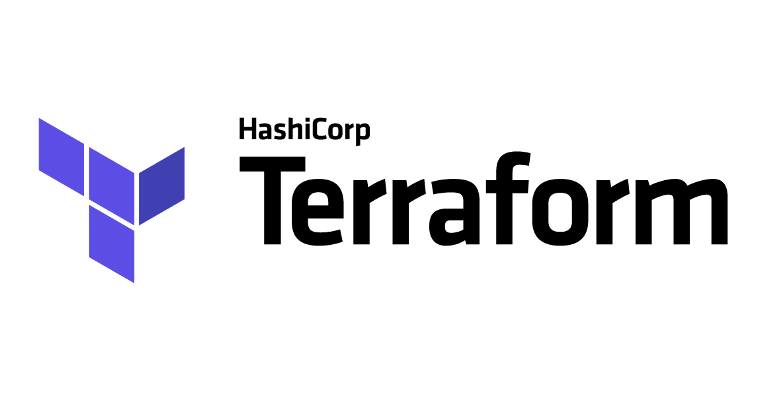
\includegraphics[width=7cm, height=4cm]{terraform.png}
    \caption{สัญลักษณ์ Terraform}
    \label{fig:Terraform-icon}
\end{figure}

% 2.4.3
\newpage
\subsection{Jenkins}
\begin{figure}[ht]
    \centering
    
\includegraphics[width=3cm, height=4cm]{jenkins.png}
    \caption{ตัวอย่างหน้าติดต่อผู้ใช้งานของระบบ Jenkins}
    \label{fig:Jenkins-UI}
\end{figure}

% 2.4.4
\newpage
\subsection{Docker}
\begin{figure}[ht]
    \centering
    
\includegraphics[width=5cm, height=5cm]{docker.png}
    \caption{สัญลักษณ์ Docker}
    \label{fig:Docker-icon}
\end{figure}

% 2.4.4
\newpage
\subsection{Jira}
\begin{figure}[ht]
    \centering
    
\includegraphics[width=5cm, height=5cm]{docker.png}
    \caption{ตัวอย่างหน้าติดต่อผู้ใช้งานของระบบ Jira}
    \label{fig:Jira-icon}
\end{figure}

% 2.4.5
\newpage
\subsection{GitLab}
\begin{figure}[ht]
    \centering
    
\includegraphics[width=7cm, height=4cm]{gitlab.png}
    \caption{สัญลักษณ์ GitLab}
    \label{fig:GitLab-icon}
\end{figure}

% 2.4.5
\newpage
\subsection{SourceTree}
\begin{figure}[ht]
    \centering
    
\includegraphics[width=7cm, height=4cm]{sourcetree.png}
    \caption{สัญลักษณ์ SourceTree}
    \label{fig:SourceTree-icon}
\end{figure}

% 2.5
\newpage
\section{ขั้นตอนการทำงาน}
\begin{enumerate}
    \item AWS ECS
    \item AWS ECR
    \item AWS EC2
    \item AWS Auto Scaling
    \item AWS Launch Configutarion
    \item AWS S3
\end{enumerate}



    \include{chapter3}
    \include{chapter4}
    \include{chapter5}

    \clearpage
    \addcontentsline{toc}{chapter}{บรรณานุกรม}
    \bibliographystyle{IEEEtran}
    \bibliography{reference}

    \startappendix
    \include{appendix}

\end{document}
